\section{The StructuralSolver framework}
In this section the \SSol{}
framework is described. In particular, after a brief overview of the
main features of this solver for structural mechanics problems, a
detailed description of the practical implementation of the different
constitutive laws is presented. In section \ref{sct-Continuum} and
\ref{sct-FEF} we have provided the complete expression for the first
Piola Kirchhoff tensor and its linearization. In this part of the
report, each of the terms that appear in the definition of \Piola and
its Jacobian, for each material law, is associated with one specific
method in the new \SSolNC{} framework. This should help the users to
work with this framework and, if needed, to reuse part of the existing
code if a new constitutive law has to be inserted in \LV.\\ The
\SSolNC{} framework has been developed in order to have a unique solver
for structural dynamic problems. The main characters which have been
introduced are:
\begin{itemize}
\item the \textit{StructuralSolver} class,
\item the \textit{StructuralMaterial} class, with the definitions of
  the constitutive laws,
\item the \textit{AssemblyElementalStructure} \texttt{namespace}.
\end{itemize}

\begin{figure}[h!]  \centering
  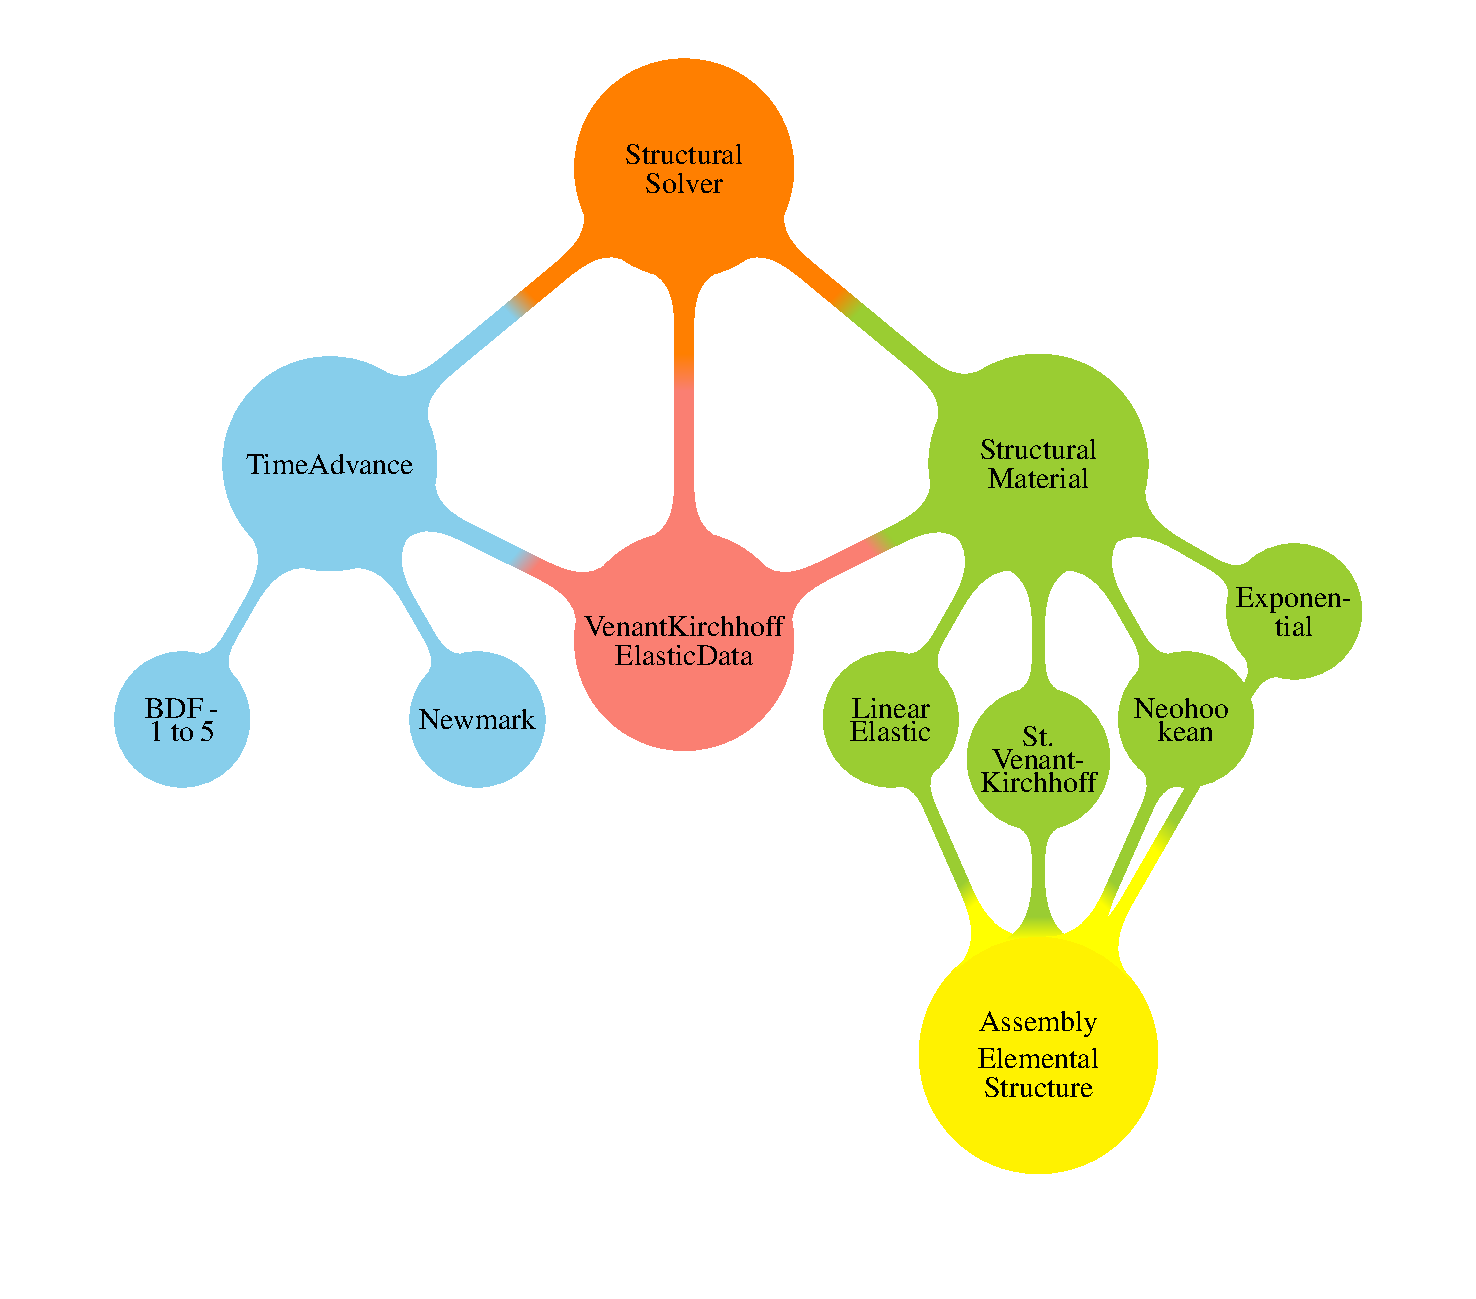
\includegraphics[width=14cm,height=12cm]{images/DesignStructural.pdf}
  \caption{Schematic representation of the main characters of the
    \SSol{} framework and of their interactions}
  \label{fig::design}
\end{figure}
\subsection{The \textit{StructuralSolver} class}
This class is the
solver of the structural mechanics problem. It has been developed
according to the common design pattern used for other solvers in
\LV. According to this, its main three methods are:
\begin{itemize}
\item \tPC{buildSystem()},
\item \tPC{updateSystem()},
\item \tPC{iterate()}.
\end{itemize}
The first builds the mass matrix \mass (which is
constant for all the time steps). The second one updates the right hand
side of the system \eqref{eq::GeneralSystem} and the last solves the
nonlinear system:
\begin{equation}
  \LE\left(\vectL^{n+1}\right)=0
  \label{eq::Root}
\end{equation}
The \tPC{iterate} method contains the Newton method
applied to \eqref{eq::Root}. The three main steps of the Newton method
are:
\begin{itemize}
\item evaluating the residual using the displacement field at the
  iteration $k$ of the Newton method. This stage is implemented in
  \tPC{StructuralSolver::evalResidual()};
\item updating the Jacobian using the displacement field at the
  current iteration $k$. It is implemented in
  \tPC{StructuralSolver::updateJacobian()};
\item solving the linearized system. The method
  \tPC{StructuralSolver::solveJacobian()} implements this stage.
\end{itemize} In order to solve the mathematical problem
\eqref{eq::MathProb}, this solver communicates with three main
classes:
\begin{itemize}
\item \tPC{StructuralMaterial},
\item \tPC{VenantKirchhoffElasticData},
\item \tPC{TimeAdvance}.
\end{itemize}
The \tPC{StructuralMaterial} class defines the
constitutive law which is used during the simulation. The second class
contains the mechanical parameters of the material (e.g. Young
modulus, Poisson ratio) and some useful variables set in the data file
of the simulation. The last class, as anticipated in \ref{sct-Linear},
manages the time advancing procedure and it is not described here.\\

\subsection{The \textit{StructuralMaterial} class} This is the core of
the new framework. It has been designed to be a general interface
between all the material models and the solver class. In this way, the
different structural models can be used in a very flexible way just
changing a variable, called solidType, in the data file.\\ For this
reason, from the practical point of view, this class is a factory (see
\cite{DesignPattern}). It has only virtual methods and the most
important are:
\begin{itemize}
\item \tPC{computeStiffness()},
\item \tPC{updateJacobianMatrix()}.
\end{itemize}
Since they are pure virtual methods, in each class
corresponding to a structural model there is the specific
implementation of the two methods above according to the chosen law.\\
The method \tPC{computeStiffness()} computes, using the displacement
fields at the iteration $k$ of the Newton method, the stiffness vector
when the solver class has to evaluate the residual in
\tPC{evalResidual()}. The second method provides StructuralSolver
with the Jacobian matrix of \Piola.\\

\subsection{The \textit{AssemblyElementalStructure}
  \texttt{namespace}}
As it will be shown later on, lots of new methods
have been developed to compute all the terms of the first
Piola-Kirchhoff tensor and its Jacobian for all the material models.
\AES{} is a new namespace defined in \LV. Its creation was necessary in
order to keep all these new methods separated from the ones which had
been previously developed (for different purposes) and grouped in the
AssemblyElemental namespace. Few methods, which were already available
in \LV{} in AssemblyElemental have been kept and not doubled in the new
namespace. When those methods are used, the interested reader may
refer to their definition in the AssemblyElemental namespace in
\tPC{AssemblyElemental.hpp}.\\ As it can be seen from
Fig. \ref{fig::design}, \AES{} is used only by the classes of the
material laws, that is where \Piola{} and the Jacobian are computed.



\subsection{Implementation of the different constitutive relations} In
this section we give a detailed description of the implementation of
the structural models. All the methods in the following receive some
arguments from the class that calls them. Here we will neglect all of
them. The interested reader may refer directly to their implementation
to have more details on this.


\subsubsection{The St. Venant-Kirchhoff model} This model is
implemented in \tPC{VenantKirchhoffMaterialNonLinear.hpp}. We will
refer to Eq. \eqref{eq::SVK-P-displ} for the definitions of the
methods.\\ The correspondance between the terms in
Eq. \eqref{eq::SVK-P-displ} and their implementation is:
\begin{itemize}
\item $\displaystyle \lambda(\diver{\displL})\I$ corresponds to
  \tPC{stiff\_div},
\item $\displaystyle \mu\big(\delOp\displL + \delOp\displL^T\big)$
  corresponds to \tPC{stiff\_strain},
\item $\displaystyle
  \frac{\lambda}{2}\big(\delOp\displL:\delOp\displL\big)$ corresponds to
  \tPC{stiff\_derdiv},
\item $\displaystyle \lambda\big(\diver{\displL}\big)\delOp\displL$
  corresponds to \tPC{stiff\_divgrad},
\item $\displaystyle
  \frac{\lambda}{2}\big(\delOp\displL:\delOp\displL\big)\delOp\displL$
  corresponds to \tPC{stiff\_gradgrad},
\item $\displaystyle \mu\big(\delOp\displL^T \delOp\displL\big)$
  corresponds to \tPC{stiff\_dergradbis},
\item $\displaystyle
  \mu\delOp\displL\big(\delOp\displL\delOp\displL^T\big)$ is splitted
  into the sum of two members. The first one corresponds to
  \tPC{stiff\_dergrad\_gradbis.} The second is
  \tPC{stiff\_dergrad\_gradbis\_Tr},
\item $\displaystyle \mu\delOp\displL\delOp\displL^T\delOp\displL$
  corresponds to \tPC{stiff\_gradgradTr\_gradbis}.
\end{itemize}
The definition of the Jacobian on \Piola{} is given in
Eq. \eqref{eq::SVK-Jacobian}. Here we specify the implementations of
the terms:
\begin{itemize}
\item $\displaystyle \lambda(\delOp\cdot\delta\Spost)$ corresponds
  to \tPC{stiff\_div},
\item $\displaystyle \mu(\delOp\delta\Spost +
  (\delOp\delta\Spost)^T)$ corresponds to \tPC{stiff\_strain},
\item $\displaystyle \lambda\delOp\Spost:\delOp\delta\Spost$
  corresponds to \tPC{stiff\_derdiv},
\item $\displaystyle \lambda(\delOp\cdot\Spost)\delOp\delta\Spost$
  corresponds to \tPC{stiff\_divgrad},
\item $\displaystyle \lambda(\delOp\cdot\delta\Spost)\delOp\Spost$
  corresponds to \tPC{stiff\_divgrad\_2},
\item $\displaystyle
  \frac{\lambda}{2}(\delOp\delta\Spost:\delOp\Spost)\delOp\Spost$ and
  the term $\displaystyle
  \frac{\lambda}{2}(\delOp\Spost:\delOp\delta\Spost)\delOp\Spost$ are
  added up in \tPC{stiff\_gradgrad\_2},
\item $\displaystyle
  \frac{\lambda}{2}(\delOp\Spost:\delOp\Spost)\delOp\delta\Spost$
  corresponds to \tPC{stiff\_gradgrad},
\item $\displaystyle \mu(\delOp\Spost)^{\text{T}}\delOp\delta\Spost$
  and the term $\displaystyle
  \mu(\delOp\delta\Spost)^{\text{T}}\delOp\Spost$ are added up and
  implemented in \tPC{stiff\_dergrad},
\item $\displaystyle \mu\delOp\Spost\delOp\delta\Spost$ corresponds
  to \tPC{stiff\_dergrad\_gradbis},
\item $\displaystyle \mu\delOp\delta\Spost\delOp\Spost$ corresponds
  to \tPC{stiff\_dergrad\_gradbis\_2},
\item $\displaystyle \mu\delOp\Spost(\delOp\delta\Spost)^{\text{T}}$
  corresponds to \tPC{stiff\_dergrad\_gradbis\_Tr},
\item $\displaystyle \mu\delOp\delta\Spost(\delOp\Spost)^{\text{T}}$
  corresponds to \tPC{stiff\_dergrad\_gradbis\_Tr\_2},
\item $\displaystyle
  \mu\delOp\delta\Spost(\delOp\Spost)^{\text{T}}\delOp\Spost$
  corresponds to \tPC{stiff\_gradgradTr\_gradbis\_3},
\item $\displaystyle
  \mu\delOp\Spost(\delOp\delta\Spost)^{\text{T}}\delOp\Spost$
  corresponds to \tPC{stiff\_gradgradTr\_gradbis\_2},
\item $\displaystyle
  \mu\delOp\Spost(\delOp\Spost)^{\text{T}}\delOp\delta\Spost$
  corresponds to \tPC{stiff\_gradgradTr\_gradbis}.
\end{itemize}


\subsubsection{The Linear Elastic model} This constitutive law is
defined in \tPC{VenantKirchhoffMaterialLinear.hpp}. We recall the
definition of \Piola{} as a function of the displacement field,
Eq. \eqref{eq::LE-P}.\\ Herein there is the list of the
correspondances:
\begin{itemize}
\item $\lambda(\diver{\displL})\I$ corresponds to the method
  \tPC{stiff\_div};
\item $\mu\big(\delOp\displL + \delOp\displL^T\big)$ corresponds to
  the method \tPC{stiff\_strain}.
\end{itemize}
In the case of linear elastic model, the Jacobian of
\Piola{} is the tensor itself and for this reason it is not
specified. The methods listed above belong to the AssemblyElemental
namespace since this constitutive law was already available in \LV{}
before the creation of the \SSolNC{} framework.


\subsubsection{The Neohookean model} The first Piola-Kirchhoff tensor
is defined in Eq. \eqref{eq::NH-P}. The terms have been implemented in
different methods as follows:
\begin{itemize}
\item $\displaystyle \mu
  J^{-\frac{2}{3}}\left(\F-\frac{1}{3}I_{\C}\F^{-T}\right)$ in the
  method \tPC{source\_P1iso\_NH},
\item $\displaystyle
  J\frac{\kappa}{2}\left(J-1+\frac{1}{J}\text{ln}J\right)\F^{-T}$ in the
  method \tPC{source\_Pvol}.
\end{itemize}
Concerning the Jacobian, defined in
Eqs. \eqref{eq::IsoPartDP-neo} and \eqref{eq::VolPartDP-neo}, the
implementation for the isochoric part has been done has follows:
\begin{itemize}
\item $\displaystyle
  -\frac{2}{3}J^{-\frac{5}{3}}\left(\cofF:\GradSpost\right)\F$ in
  \tPC{stiff\_Jac\_P1iso\_NH\_1term},
\item $\displaystyle \frac{2}{9}\mu
  J^{-2}I_{\C}\left(\cofF:\GradSpost\right)\cofF$ in
  \tPC{stiff\_Jac\_P1iso\_NH\_2term},
\item $\displaystyle \frac{2}{3}\mu
  J^{-\frac{5}{3}}\left(\F:\GradSpost\right)\cofF$ in
  \tPC{stiff\_Jac\_P1iso\_NH\_3term},
\item $\displaystyle \mu J^{-\frac{2}{3}}\GradSpost$ in
  \tPC{stiff\_Jac\_P1iso\_NH\_4term},
\item $\displaystyle
  \frac{\mu}{3}J^{-2}I_{\C}\cofF\GradSpost^T\cofF$ in
  \tPC{stiff\_Jac\_P1iso\_NH\_5term}.
\end{itemize}
For the volumetric part, these methods have been
created:
\begin{itemize}
\item $\displaystyle
  \frac{\kappa}{2}\left(2J^2-J+1\right)\left[\F^{-T}:\GradSpost\right]\F^{-T}$
  in \tPC{stiff\_Jac\_Pvol\_1term},
\item $\displaystyle
  \frac{\kappa}{2}\left(J-J^2-\text{ln}(J)\right)\F^{-T}\GradSpost^T\F^{-T}$
  in \tPC{stiff\_Jac\_Pvol\_2term}.
\end{itemize}


\subsubsection{The Exponential model} In this case we analyze only the
isochoric part of \Piola{} (Eq. \eqref{eq::EXP-P}). It is composed only
by one term,
\begin{displaymath}
  \displaystyle \alpha
  J^{-\frac{2}{3}}\left(\F-\frac{1}{3}I_{\C}\F^{-T}\right)
  e^{\gamma\big(I_{\C}-3\big)},
\end{displaymath}
and it has been implemented in the method
\tPC{source\_P1iso\_Exp}.  The correspondance between the terms of the
isochoric part of the Jacobian (Eq. \eqref{eq::IsoPartDP-exp}) and
their own implementations in AssemblyElementalStructure is:
\begin{itemize}
\item $\displaystyle -\frac{2}{3}\alpha\term
  J^{-\frac{5}{3}}\left(1+\gamma
    I_{\C}\right)\left[\cofF:\GradSpost\right]\F$ corresponds to
  \tPC{stiff\_Jac\_P1iso\_Exp\_1term},
\item $\displaystyle 2\alpha\gamma\term J
  ^{-\frac{4}{3}}\left(\F:\GradSpost\right)\F$ corresponds to
  \tPC{stiff\_Jac\_P1iso\_Exp\_2term},
\item $\displaystyle \frac{2}{9}\alpha\term
  J^{-2}I_{\C}\left(1+\gamma
    I_{\C}\right)\left(\cofF:\GradSpost\right)\cofF$ corresponds to
  \tPC{stiff\_Jac\_P1iso\_Exp\_3term},
\item $\displaystyle -\frac{2}{3}\alpha\term
  J^{-\frac{5}{3}}\left(1+\gamma
    I_{\C}\right)\left(\F:\GradSpost\right)\cofF$ corresponds to
  \tPC{stiff\_Jac\_P1iso\_Exp\_4term},
\item $\displaystyle \alpha\term J^{-\frac{2}{3}}\GradSpost$
  corresponds to \tPC{stiff\_Jac\_P1iso\_Exp\_5term},
\item $\displaystyle \frac{\alpha}{3}\term
  J^{-2}I_{\C}\cofF\GradSpost^T\cofF$ corresponds to
  \tPC{stiff\_Jac\_P1iso\_Exp\_6term}.
\end{itemize}
The volumetric part in both the first Piola-Kirchhoff
tensor and in its Jacobian, is the same for the Neohookean and
Exponential model. For this reason, it has not been specified here.
